\chapter{Constrains using HAWC on GRB170817A}

Desafortunadamente, el evento de la onda gravitacional GW170817 ocurri� fuera del campo de visi�n de HAWC. Sin embargo, 8 hrs depu�s el tr�nsito logra entrar en el campo de visi�n del observatorio colocando un upper limit a XX \citep{2017ApJ...848L..12A}. Debido a la naturaleza que present� el afterglow de este GRB, en donde, apareci� la emisi�n de rayos X a 9 d�as \textbf{[??]} y de radio a 16 d�as \textbf{[??]} despu�s del destello respectivamente, alcanzando un flujo m�ximo a los \textcolor{red}{120 d�as} \textbf{[??]} se realiza un monitoreo a ciegas buscando  emisi�n en TeV's detectable por HAWC.

\section{Mapas del cielo de d�as siderales}

HAWC presenta su �ptima sensibilidad para fuentes que se encuentran dentro de las declinaciones -26$\degree$ y +64$\degree$, tal y como se muestra la regi�n sombreada en la figura \ref{fig:FOV-HAWC}. De esta manera definimos a un transito como la visibilidad de una fuente por HAWC la cual se encuentra con un �ngulo cenital $\theta$ < 45$\degree$ .

\begin{figure}[ht!]
  \centering{
  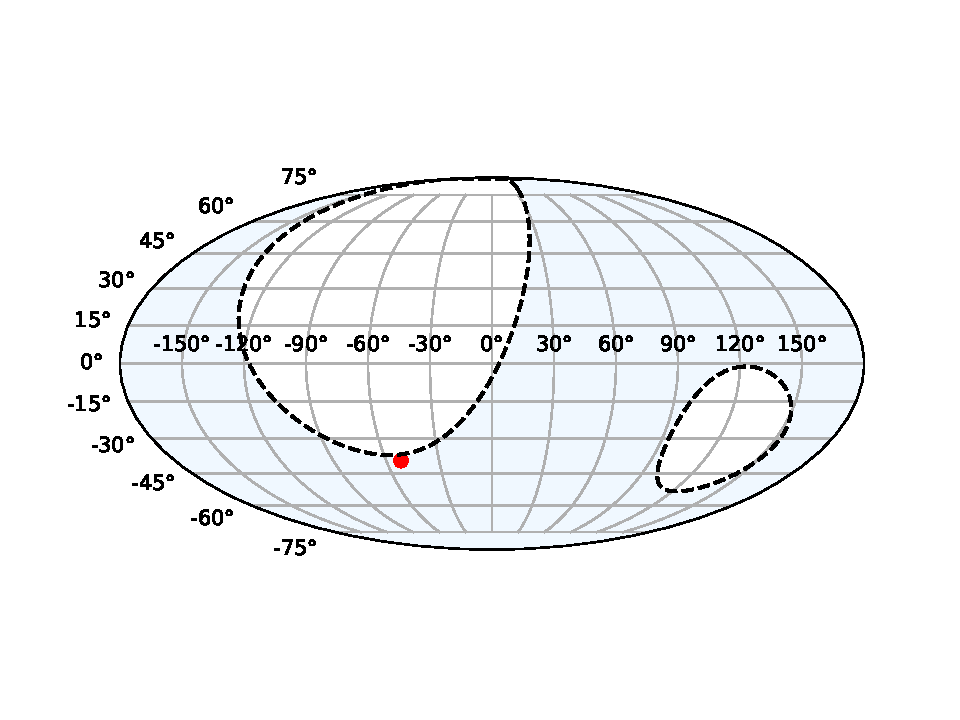
\includegraphics[width=1.0\linewidth]{Figures/HAWC_GW.pdf}}
  \caption{Campo de visi�n de HAWC}
  \label{fig:FOV-HAWC}
\end{figure}

\section{B�squeda tard�a en TeVs}
Considerando bines temporales de...